%% ICPC/TopCoder/CodeForces 상위랭커 
%% http://k2code.blogspot.kr/2012/01/given-integer-array-and-number-x-find.html

\documentclass{article}

\usepackage{amsmath, amssymb}
\usepackage{fullpage}
\usepackage{listings}% http://ctan.org/pkg/listings
\lstset{
  basicstyle=\ttfamily,
  mathescape
}
\usepackage{times}
\usepackage{url}
\usepackage[colorlinks=true, linkcolor=blue,]{hyperref}
\usepackage{xcolor}
\usepackage{tikz,subfig}
\usetikzlibrary{topaths}
\usetikzlibrary{calc, arrows}
\tikzset{
  treenode/.style = {align=center, inner sep=0pt, text centered,
    font=\ttfamily},
  arn_n/.style = {treenode, circle, draw=black,
    text width=1.5em},% arbre rouge noir, noeud noir
  arn_r/.style = {treenode, circle, red, draw=red, 
    text width=1.5em, very thick},% arbre rouge noir, noeud rouge
  arn_x/.style = {treenode, rectangle, draw=black,
    minimum width=0.5em, minimum height=0.5em}% arbre rouge noir, nil
}

\newcommand{\Z}{\mathbb{Z}}
\newcommand{\dv}{{\mathrm{div}}}
\newcommand{\md}{{\mathrm{mod}}}
\newcommand{\lcm}{{\mathrm{lcm}}}

\newtheorem{df}{Definition}[section]

\date{March 5, 2018}
\title{The 4\textsuperscript{th} Problem Set}

\begin{document}
\maketitle
\section*{Pre-requisites}
You should do the followings
\begin{enumerate}
\item On a separate and clean paper,  you need to describe your own strategy to solve the problems below, and 
	to justify why your strategy is effective while handling each problem
\item On a new clean paper, transform your strategy into an algorithm, using your own form to express algorithms.
	Further, you need to analyze the total running steps of your algorithm and the required memory amount to finish your algorithm.
	Then express the total costs using Big-O notation.
\item Use the \texttt{Code ocean} (\url{https://codeocean.com}) platform; if necessary, you may invite me using my email address 
\texttt{lightsun.kim@gmail.com}.
\item Time limits for each problem
\begin{itemize}
\item Problem \#1: Within 4 hours
\item Problem \#2: Within 3 hours
\item Problem \#3: Within 3 hours
\end{itemize}
Then you need to prepare two answer codes; one is a C code that you have made within each time limit, and the
other is a C code augmented and fixed from the original code later.
\end{enumerate}

\newpage

\section{Problem \#1}

Let $n$ be a positive integer and a set $X=\{1,2,\ldots,5n\}$.
Assume that you are given an integer $\alpha$ and an integer array $A=\langle a_1,a_2,\ldots,a_n\rangle$  
whose element $a_i\in X$ for each $1\leq i\leq n$. Your goal in this problem is to implement an efficient algorithm 
for determining whether the set $A$ has two elements $a_i\in A$ and $a_j\in A$ 
such that $\alpha=a_i+a_j$, for $1\leq i\neq j\leq n$.  A simple solution for this problem is the algorithm $\mathtt{Exhaustive}(A,n,\alpha)$ below. 
This naive algorithm is trying to exhaustively look into all possible pairs from $A$.

\begin{table}[h]
\centering
\begin{tabular}{lrlllll}\hline
\multicolumn{7}{l}{\textsf{Algorithm} $\mathtt{Exhaustive}(A,n,\alpha)$} \\ \hline
\multicolumn{7}{l}{INPUT: An $n$-element integer array $A=\langle a_1,\ldots,a_n\rangle$ whose elements are in $X$}\\
& & \multicolumn{5}{l}{where $X=\{1,2,\ldots,5n\}$ for some positive integer $n$.}\\
\multicolumn{7}{l}{OUTPUT: A pair of indices $(i,j)$ such that $\alpha=a_i+a_j$ if exists; otherwise $\perp$} \\ 
&1. & \multicolumn{5}{l}{\textbf{for} $i\gets 1$ \textbf{to} $n$}\\
&2. & & \multicolumn{4}{l}{\textbf{for} $j\gets 1\wedge j\neq i$ \textbf{to} $n$}\\
&  3. &  & &\multicolumn{3}{l}{\textbf{if} $a_i+a_j=\alpha$ \textbf{then}}\\
&  4. &  & & & \multicolumn{2}{l}{\textbf{return} $(i,j)$}\\
&5. &  \multicolumn{5}{l}{\textbf{return} $\perp$}\\\hline
\end{tabular}
\end{table}

This algorithm will work correctly; however it requires $O(n^2)$ run-time complexity and thus 
when $n$ is a huge-sized integer (e.g., $n=10^{20}$) it shows a very slow execution time.
Thus your technical mission is to improve this algorithm in a stepwise manner.
To do this, firstly you need to  find a somewhat improved algorithm $\mathtt{Somewhat}(A,n,\alpha)$ whose run-time 
complexity is $O(n\log n)$. Next, you should devise a significantly improved algorithm 
$\mathtt{Significant}(A,n,\alpha)$ whose run-time complexity is merely $O(n)$.
Moreover, in order to argue that your idea is effective so as to improve the run-time complexity,
you should measure running times of all three programs in milliseconds over $10^{6}$ randomly generated samples.
All sampled elements are positive integers at most of 22 bits.



\bigskip
\noindent\textbf{Language requirements. }%
During tackling this problem, you should follow the programming rules:
\begin{itemize}
\item You should use an ANSI C programming language whose source code can run on \texttt{Code ocean} platform. 
\item Function naming: Begin with the lower character, and every parameters are strong-typed variables (i.e., do not use \texttt{void} typed variables).
	All functions should have a single return value; thus even if a function will return no values; you should provide \texttt{return} keyword.
\item Variable naming: Begin with a type-discriminating prefix. For example, if a variable name is for an age and is with an integer type,
	you need to declare the variable as \texttt{int iAge;}  Especially for string-type variables you are strongly recommended to use the prefix \texttt{sz}.
	For example, if a variable name is for a name, then \texttt{szName} is a preferable choice.
\end{itemize}

\bigskip
\noindent\textbf{Input format.} %
The input is given a text-format file, named \texttt{input.txt} and all strings are separated by commas.
The file contains $10^6$ integers, $A=(a_1,a_2,\ldots,a_{10^6})$, which have been randomly generated prior to execution, and
each $a_i$ is in the range of $1$ and $2^{22}$. You see that $n=10^6$ and because $10^6\approx 2^{20}$ you have $5n\approx 2^{22}$.
Note that the input file does not include the size of the array $A$; thus the input file is given in form as follows:
\begin{lstlisting}[backgroundcolor=\color{yellow!40}]
$a_1,a_2,\ldots,a_{1000}$
$a_{1001},a_{1002},\ldots,a_{2000}$
$\cdots$
$a_{999001},a_{999002},\ldots,a_{10^6}$
\end{lstlisting}



\bigskip
\noindent\textbf{Output format.} %
The output should be given as a text-format file, named \texttt{output.txt}.
The output file writes (1) the pair of indices $(i,j)$ if exists; otherwise $(0,0)$ indicating there are no matching indices
(2) if exists, the solution $\alpha=a_i+a_j$, else skip this line and (3) the execution times of your each algorithm. 

\begin{lstlisting}[backgroundcolor=\color{yellow!40}]
***************************************
(1) By my exhaustive algorithm
***************************************
$(i,j)$=(i,j)
$\alpha$=$a_i$+$a_j$ 
The total execution time: ______ sec

***************************************
(2) By my somewhat improved algorithm
***************************************
$(i,j)$=(i,j)
$\alpha$=$a_i$+$a_j$ 
The total execution time: ______ sec

***************************************
By my significantly improved algorithm
***************************************
$(i,j)$=(i,j)
$\alpha$=$a_i$+$a_j$ 
The total execution time: ______ sec
\end{lstlisting}
 
 
\newpage
\section{Problem \#2}

Regarding a binary tree $T$, we follow the usual terminologies such as binary trees, root, child/parent nodes, height and so on~\cite[\S5.1,\S5.2]{HSAf08}.
Especially we define ancestor and descendent nodes in order to avoid any type of ambiguity as follows.
\begin{df}[Ancestors, Descendants]
Let $\alpha,\beta$ be nodes of a binary tree $T$.
$\alpha$ is an ancestor of  $\beta$ if $\alpha$ is a parent of $\beta$, or
$\alpha$ is the ancestor of the parent of $\beta$. 
Further, $\alpha$ is descendant of $\beta$ if $\alpha$ is a child of $\beta$, or
$\alpha$ is a descendant of a child of $\beta$.
\end{df}

Let $T$ be a binary node with $N$ nodes. 
Keeping in mind these terms, we define a \textbf{roman node} of order $d$ by a node $\alpha\in T$
such that the number of descendants in $\alpha$'s left subtree differ from the number of 
descendants of $\alpha$'s right subtree by at most $d$.
More formally, for a node $\alpha\in T$ let $\alpha_L,\alpha_R$ be the left and right nodes of $\alpha$, respectively.
Then let $T_L(\alpha),T_R(\alpha)$ be binary trees whose roots are $\alpha_L$ and $\alpha_R$, respectively.
Writing $T_L(\alpha)=\{u_1,\ldots,u_n\}$ and $T_R(\alpha)=\{v_1,\ldots,v_m\}$ for some integers $n,m\leq N$,
if $\alpha$ is a roman node of order $d$, then $|n-m|\leq d$.
This problem requires that you should implement a C program  so that 
it finds each node $\alpha$ of $T$ such that $\alpha$ is not a roman node of order $d$, but
all of $\alpha$'s descendants are roman nodes of order $d$. 
Furthermore your algorithm for this program should satisfy $O(N)$ run-time complexity.
You may get some idea from Problem \#3 in the next pape.
 
 
\bigskip
\noindent\textbf{Input format.} %
The input is given a text-format file, named \texttt{input.txt} and all strings are separated by blanks.
\begin{lstlisting}[backgroundcolor=\color{yellow!40}]
rn=$\alpha$,d=$d$
$\ell_1$
$\ell_2\ \ell_3$
$\cdots$
$\ell_{2^{t-1}},\ell_{2^{t-1}+1},\ldots,\ell_{2^t-1}$
\end{lstlisting}
Here the first line means that $\alpha$ is the label name of roman node and $d$ is the order of $\alpha$.
A binary tree $T$ of height $t$ is described from the second line to the end line.
As you expected, the second line shows the label name of the root node of $T$ and 
its below line consists of its left child node and right child node. 
Every label name consists of a single lowercase alphabet followed by a non-zero integer, 
for example, \texttt{u9}, \texttt{v12}, or \texttt{a09}.
If its left/right children do not exits, the symbol `$\ast$' is placed at its corresponding position.  
Thus each $\ell_i$ means either a label name or the empty child node ($\ast$).
For example, consider the following binary tree.
 
\begin{figure}[h]
\centering
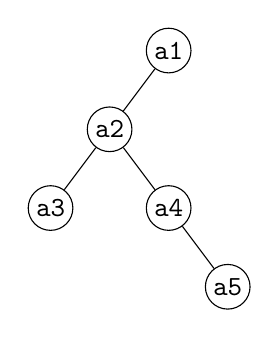
\begin{tikzpicture}[level/.style={sibling distance=15mm, level distance = 10mm}]

\node[arn_n]  (a1) {a1}
	child {node[arn_n] (a2) {a2}
		child{node[arn_n] (a3) {a3}
		}
		child{node[arn_n] (a4) {a4}
			child[missing]
			child{node[arn_n] (a5) {a5}
			}
		}
	}
	child[missing];
\end{tikzpicture}
\end{figure} 

The following shows a part of  \texttt{input.txt} for the tree as above
\begin{lstlisting}[backgroundcolor=\color{yellow!40}]
$\cdots$
a1
a2 $\ast$
a3 a4 $\ast$ $\ast$
$\ast$ $\ast$ $\ast$ a5 $\ast$ $\ast$ $\ast$ $\ast$
\end{lstlisting}
 

\bigskip
\noindent\textbf{Output format.} %
The output should be given as a text-format file, named \texttt{output.txt}.
The output file writes the resulting roman nodes of order $d$.
%$d=\gcd(a,b)$ and $m^\ast=\lcm(a^\ast,b^\ast)$ under the condition described as above.
% 
\begin{lstlisting}[backgroundcolor=\color{yellow!40}]
$\alpha_1,\cdots, \alpha_w$
\end{lstlisting}
%
%%
%% 
\newpage
\section{Problem \#3} 

Roughly speaking, there are dozens of traversal methods of a binary tree. Some of well-known tree traversals include pre-order, post-order, 
in-order. 
An important application of tree traversal is to evaluate an arithmetic express $E$ without considering parentheses included in $E$.
For example, consider an arithmetic expression
\begin{align*}
E=((((3+1)\ast 3)/((9-5)+2))-((3\ast(7-4))+6)).
\end{align*}
This expression can be represented as a proper binary tree as follows.
\begin{figure}[h]
\centering
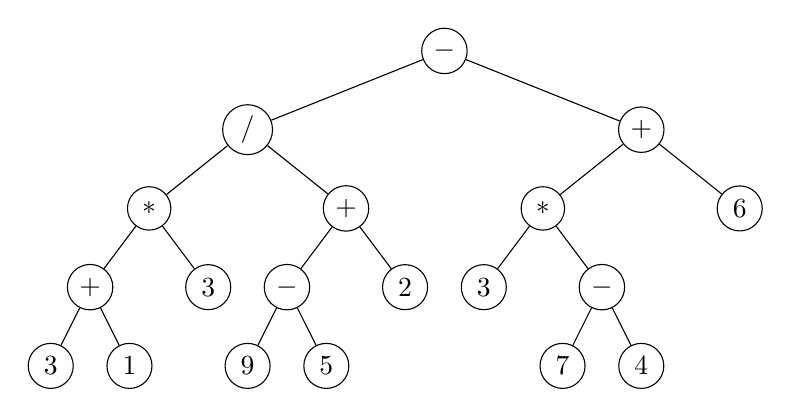
\begin{tikzpicture}[level 1/.style={sibling distance=50mm}, level 2/.style={sibling distance=25mm}, level 3/.style={sibling distance=15mm}, 
	level 4/.style={sibling distance=10mm}, level distance = 10mm]

\node[arn_n]  (a1) {$-$}
	child {node[arn_n] (a2) {$/$}
		child{node[arn_n] (a3) {$\ast$}
			child{node[arn_n] (a7) {$+$}
				child{node[arn_n] (a9) {$3$}}
				child{node[arn_n] (a10){$1$}}
			}
			child{node[arn_n] (a8) {$3$}
			}
		}
		child{node[arn_n] (a4) {$+$}
			child{node[arn_n] (a11) {$-$}
				child{node[arn_n] (a12) {$9$}}
				child{node[arn_n] (a19) {$5$}}
			}
			child{node[arn_n] (a5) {$2$}}
		}
	}
	child{node[arn_n] (a6) {$+$}
		child{node[arn_n] (a13) {$\ast$}
			child{node[arn_n] (a15) {$3$}}
			child{node[arn_n] (a16) {$-$}
				child{node[arn_n] (a17) {$7$}}
				child{node[arn_n] (a18) {$4$}}
			}
		}
		child{node[arn_n] (a14) {$6$}}
	};
%\draw[->,bend right =15,thick,red] (a9.east) to (a7.south);
\end{tikzpicture}
\end{figure} 

Then evaluating the arithmetic express $E$ by the inorder traversal is performed as follows:
\begin{figure}[h]
\centering
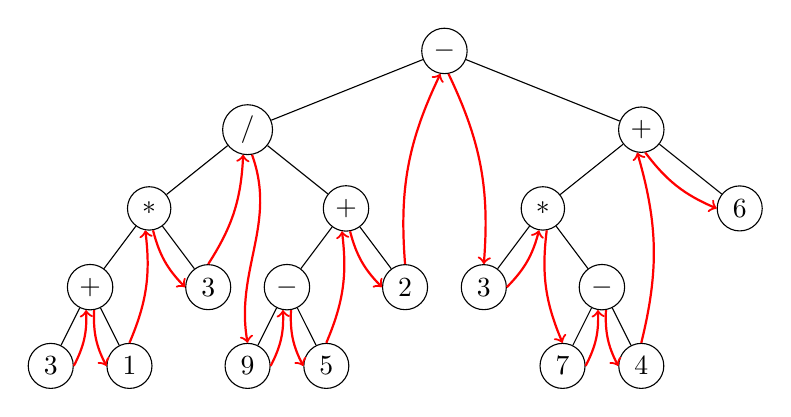
\begin{tikzpicture}[level 1/.style={sibling distance=50mm}, level 2/.style={sibling distance=25mm}, level 3/.style={sibling distance=15mm}, 
	level 4/.style={sibling distance=10mm}, level distance = 10mm]

\node[arn_n]  (a1) {$-$}
	child {node[arn_n] (a2) {$/$}
		child{node[arn_n] (a3) {$\ast$}
			child{node[arn_n] (a7) {$+$}
				child{node[arn_n] (a9) {$3$}}
				child{node[arn_n] (a10){$1$}}
			}
			child{node[arn_n] (a8) {$3$}
			}
		}
		child{node[arn_n] (a4) {$+$}
			child{node[arn_n] (a11) {$-$}
				child{node[arn_n] (a12) {$9$}}
				child{node[arn_n] (a19) {$5$}}
			}
			child{node[arn_n] (a5) {$2$}}
		}
	}
	child{node[arn_n] (a6) {$+$}
		child{node[arn_n] (a13) {$\ast$}
			child{node[arn_n] (a15) {$3$}}
			child{node[arn_n] (a16) {$-$}
				child{node[arn_n] (a17) {$7$}}
				child{node[arn_n] (a18) {$4$}}
			}
		}
		child{node[arn_n] (a14) {$6$}}
	};
\draw[->,bend right =15,thick,red] (a9.east) to (a7.260);
\draw[->,bend right =15,thick,red] (a7.280) to (a10.west);
\draw[->,bend right =15,thick,red] (a10.north) to (a3.260);
\draw[->,bend right =15,thick,red] (a3.280) to (a8.west);
\draw[->,bend right =15,thick,red] (a8.north) to (a2.260);
\draw[->,thick,red] (a2.280) to[out=290,in=100] (a12.north);
\draw[->,bend right =15,thick,red] (a12.east) to (a11.260);
\draw[->,bend right =15,thick,red] (a11.280) to (a19.west);
\draw[->,bend right =15,thick,red] (a19.north) to (a4.260);
\draw[->,bend right =15,thick,red] (a4.280) to (a5.west);
\draw[->,bend left =15,thick,red] (a5.north) to (a1.260);
\draw[->,bend left =15,thick,red] (a1.280) to (a15.north);
\draw[->,bend right =15,thick,red] (a15.east) to (a13.260);
\draw[->,bend right =15,thick,red] (a13.280) to (a17.north);
\draw[->,bend right =15,thick,red] (a17.east) to (a16.260);
\draw[->,bend right =15,thick,red] (a16.280) to (a18.west);
\draw[->,bend right =15,thick,red] (a18.north) to (a6.260);
\draw[->,bend right =15,thick,red] (a6.280) to (a14.west);
\end{tikzpicture}
\end{figure} 

To the contrary, this problem considers an operation in this opposite direction.
This is to say, given a binary tree $T$ representing an arithmetic expression
you are required to print the expression $E$ by reading the tree $T$.
One popular way to do this task is to use a tree traversal known as the \textbf{Euler tour traversal}.

Roughly, the Euler tour traversal of a binary tree $T$ can be considered as a ``walk'' around the tree $T$,
where start by going from the root $r$ towards its left child $T_L(r)$, thinking of the edges of $T$ as being 
``walks'' that you always keep to your left. Refer to Figure \ref{fig:euler}, in the next page. 
Yo can see that you stop by each node $v\in T$ three times by the Euler tour which consists of three basic operations:
\begin{enumerate}
\item Left visit. You will see $v$ before the Euler tour of $v$'s left subtree $T_L(v)$. Denote it by $\mathtt{left}(v)$.
\item Below visit. You will also see $v$ immediately after the Euler tour of $v$'s two subtrees). Denote it by $\mathtt{below}(v)$.
\item Right visit. You will see again $v$ after the Euler tour of $v$'s right subtree $T_R(v)$. Denote it by  $\mathtt{right}(v)$.
\end{enumerate}

You may observe that if $v$ is an external node, then those three visiting operations all happen at the same time.
Thus the Euler tour traversal is a generalization of pre-order, in-order, and post-order traversals. 
In other words, the pre-order traversal of $T$ is equivalent to an Euler tour traversal such that
each node has an associated ``visit'' operation occur only when 
it is encountered on the left.
Similarly, the in-order and post-order traversals of $T$ are equivalent to an Euler tour traversal such that 
each node has an associated ``visit'' operation occur only when it is encountered from below or on the right, respectively.
 
\begin{figure}[h]
\centering
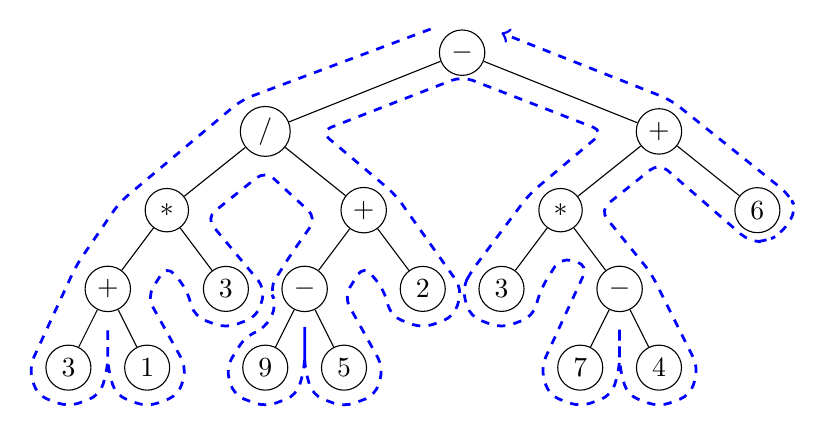
\begin{tikzpicture}[level 1/.style={sibling distance=50mm}, level 2/.style={sibling distance=25mm}, level 3/.style={sibling distance=15mm}, 
	level 4/.style={sibling distance=10mm}, level distance = 10mm,
	%scale=0.7, transform shape
]

\node[arn_n]  (a1) {$-$}
	child {node[arn_n] (a2) {$/$}
		child{node[arn_n] (a3) {$\ast$}
			child{node[arn_n] (a7) {$+$}
				child{node[arn_n] (a9) {$3$}}
				child{node[arn_n] (a10){$1$}}
			}
			child{node[arn_n] (a8) {$3$}
			}
		}
		child{node[arn_n] (a4) {$+$}
			child{node[arn_n] (a11) {$-$}
				child{node[arn_n] (a12) {$9$}}
				child{node[arn_n] (a19) {$5$}}
			}
			child{node[arn_n] (a5) {$2$}}
		}
	}
	child{node[arn_n] (a6) {$+$}
		child{node[arn_n] (a13) {$\ast$}
			child{node[arn_n] (a15) {$3$}}
			child{node[arn_n] (a16) {$-$}
				child{node[arn_n] (a17) {$7$}}
				child{node[arn_n] (a18) {$4$}}
			}
		}
		child{node[arn_n] (a14) {$6$}}
	};
\draw[->, blue, rounded corners, dashed, line width=1pt] 
($(a1)+(-0.4,0.3)$) -- ($(a2) +(-0.3,0.4)$) -- ($(a3) +(-0.6,0.1)$) -- ($(a7)  +(-0.4,0.3)$) -- 
($(a9)  +(-0.5,0.0)$) -- ($(a9)  +(-0.4,-0.35)$) -- ($(a9)  +(0.0,-0.5)$) -- ($(a9)  +(0.4,-0.35)$) --  ($(a9)  +(0.5,0.0)$) --  ($(a7)  +(0.0,-0.4)$) --
($(a10)  +(-0.5,0.0)$) --  ($(a10)  +(-0.4,-0.35)$) -- ($(a10)  +(0.0,-0.5)$) --  ($(a10)  +(0.4,-0.35)$) --  ($(a10)  +(0.5,0.0)$) --
($(a7)  +(0.5,-0.1)$) --  ($(a3)  +(0.0,-0.7)$) -- ($(a8)  +(-0.5,0.0)$) -- ($(a8)  +(-0.4,-0.35)$) -- ($(a8)  +(0.0,-0.5)$) --
($(a8)  +(0.4,-0.35)$) -- ($(a8)  +(0.5,0.0)$) -- ($(a3)  +(0.5,-0.1)$) -- ($(a2)  +(0.0,-0.5)$) -- ($(a4)  +(-0.6,-0.1)$) --
($(a11)  +(-0.2,0.4)$) -- ($(a11)  +(-0.45,0.0)$) -- ($(a11)  +(-0.35,-0.2)$) -- ($(a12)  +(0.0,0.5)$) -- ($(a12)  +(-0.25,0.4)$) --
($(a12)  +(-0.5,0.0)$) -- ($(a12)  +(-0.4,-0.35)$) -- ($(a12)  +(0.0,-0.5)$) -- ($(a12)  +(0.4,-0.35)$) -- ($(a12)  +(0.5,0.0)$) --
($(a11)  +(0.0,-0.4)$) -- ($(a19)  +(-0.5,0.0)$) --
($(a19)  +(-0.5,0.0)$) -- ($(a19)  +(-0.4,-0.35)$) -- ($(a19)  +(0.0,-0.5)$) -- ($(a19)  +(0.4,-0.35)$) -- ($(a19)  +(0.5,0.0)$) --
($(a11)  +(0.5,-0.1)$) --  ($(a4)  +(0.0,-0.7)$) -- ($(a5)  +(-0.5,0.0)$) -- ($(a5)  +(-0.4,-0.35)$) -- ($(a5)  +(0.0,-0.5)$) --
($(a5)  +(0.4,-0.35)$) -- ($(a5)  +(0.5,0.0)$) -- ($(a4)  +(0.4,0.2)$) -- ($(a2)  +(0.7,0.0)$) --
($(a1)  +(0.0,-0.3)$) -- ($(a6)  +(-0.7,0.0)$) -- ($(a13)  +(-0.4,0.2)$) -- ($(a15)  +(-0.4,0.2)$) --
($(a15)  +(-0.5,0.0)$) --  ($(a15)  +(-0.4,-0.35)$) -- ($(a15)  +(0.0,-0.5)$) --  ($(a15)  +(0.4,-0.35)$) --  ($(a15)  +(0.5,0.0)$) --
 ($(a13)  +(0.0,-0.6)$) -- ($(a16)  +(-0.4,0.3)$) -- 
($(a17)  +(-0.5,0.0)$) -- ($(a17)  +(-0.4,-0.35)$) -- ($(a17)  +(0.0,-0.5)$) -- ($(a17)  +(0.4,-0.35)$) --  ($(a17)  +(0.5,0.0)$) --  ($(a16)  +(0.0,-0.4)$) --
($(a18)  +(-0.5,0.0)$) --  ($(a18)  +(-0.4,-0.35)$) -- ($(a18)  +(0.0,-0.5)$) --  ($(a18)  +(0.4,-0.35)$) --  ($(a18)  +(0.5,0.0)$) --
($(a16)  +(0.4,0.2)$) --   ($(a13)  +(0.5,0.0)$) -- ($(a6)  +(0.0,-0.4)$) -- ($(a14) +(-0.1,-0.4)$) -- ($(a14) +(0.1,-0.4)$) --
($(a14) + (0.3,-0.3)$) -- ($(a14) + (0.5,0.0)$) --  ($(a14) + (0.4,0.2)$) -- ($(a6) + (0.15,0.4)$) --  ($(a1) + (0.5,0.25)$) ;
\end{tikzpicture}
\caption{Euler tour traversal of a binary tree}\label{fig:euler}
\end{figure}  

\bigskip
The goal in this problem is simply to implement a C program to print a fully parenthesized arithmetic expression $E$ from its 
representing binary tree $T$. Your program should implement and invoke the three Euler tour operations $\mathtt{left}(),\mathtt{below}()$, and $\mathtt{right}()$, properly.
Assume that you have only six arithmetic operations $+,-,{\ast},/$, {\textasciicircum}, and $\%$.

\bigskip
\noindent\textbf{Input format.} %
The input is given a text-format file, named \texttt{input.txt}. This file describes a binary tree $T$ of $N$ nodes in the level-order manner where each node $v$ is 
written by $v=[u_{i1},u_{i2},u_{i3}]$ for the label name of $v$ and its left/right children $u_{i2},u_{i3}$, respectively.
Indicating a node without children is by \#.
\begin{lstlisting}[backgroundcolor=\color{yellow!40}]
[$u_{11}$,$u_{12}$,$u_{13}$]
[$u_{21}$,$u_{22}$,$u_{23}$]
$\cdots$
[$u_{N1}$,$u_{N2}$,$u_{N3}$]
\end{lstlisting}
For example,  the binary tree in Figure~\ref{fig:euler} is given by
\begin{lstlisting}[backgroundcolor=\color{white}]
[-,/,+]
[/,*,+]
[+,*,6]
[*+,3]
[+,-,2]
[*,3,-]
[6,#,#]
[+,3,1]
[3,#,#]
[-,9,3]
[2,#,#]
[3,#,#]
[-,7,4]
[3,#,#]
[1,#,#]
[9,#,#]
[5,#,#]
[7,#,#]
[4,#,#]
\end{lstlisting}


\bigskip
\noindent\textbf{Output format.} %
The output should be given as a text-format file, named \texttt{outputc.txt}, \texttt{outputq.txt}, or \texttt{outputl.txt}.
The output file writes a fully parenthesized arithmetic expression.

\begin{lstlisting}[backgroundcolor=\color{yellow!40}]
$\ast\ast$ The arithmetic expression $\ast\ast$
$E=$
\end{lstlisting}

\newpage
\begin{thebibliography}{100}
%\addtolength{\leftmargin}{0.2in}
%\setlength{\itemindent}{-0.2in}

\bibitem[HSAf08]{HSAf08} E. Horowitz, S. Sahni, and S. Anderson-Free, \emph{Fundamentals of Data Structures in C}, Second edition, Silicon Press, 2008. 


%\bibitem[Jos27]{Jos27}  Flavius Josephus, \emph{The jewish war  Book III},  Translated by H. S. Thackeray,  Heinemann 1927,
%342--366 \& 387--391.
 \end{thebibliography}            
\end{document}

 


































